%!TEX root = ../thesis.tex

% *****************************************************************************
% ********************************** CHAPTER 2 ********************************
% *****************************************************************************

\chapter{Board Characteristics}

\section{Board Selection}

\section{Introduction to AM64x}

AM64x is an extension of the Sitara industrial-grade family of heterogeneous
Arm processors. \cite{AM64_datasheet}
AM64x is designed for applications in industrial automation, industrial
communication, and other embedded systems application which require a unique
combination of real-time processing and communications with application
processing. 

AM64x combines two instances of Sitara's gigabit TSN-enabled PRU-ICSSG,
two Arm Cortex-A53 cores, four Cortex-R5F MCUs, and a Cortex-M4F MCU
domain.

\begin{figure}[htb]
    \centering
    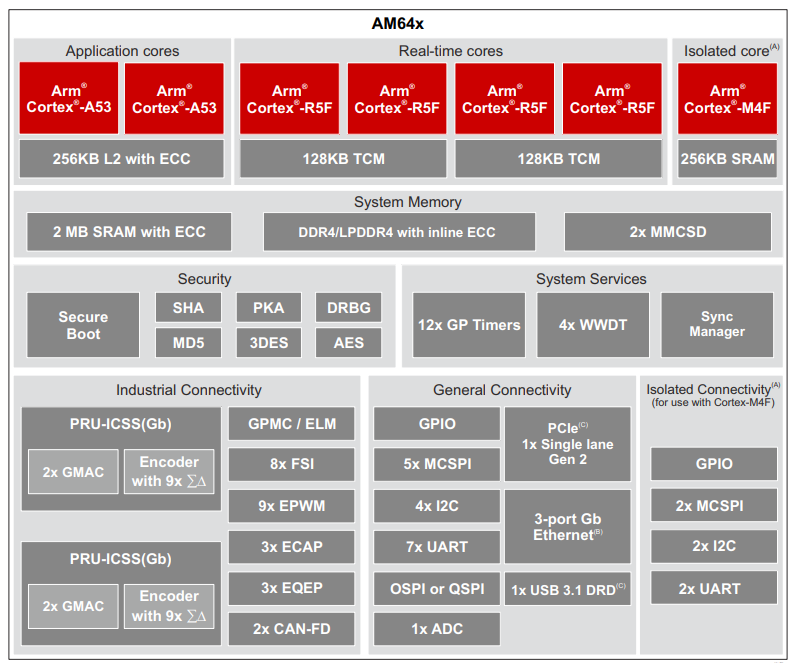
\includegraphics[width=1.0\textwidth]{am64_architecture.png}
    \caption{AM64x architecture}
\end{figure}

The Arm Cortex-A53 Cores are specifically optimized for higher-level
processing tasks.
They offer good performance for general-purpose computing and serving as a
popular choice for running operating systems, such as embedded Linux.
Their computational power enables the fusion of the Linux environment with the
real-time capabilities offered by the other cores within the AM64x.
The AM64x offers configurable memory partitioning, facilitating the division
of memory allocation between the Linux cores and the real-time cores.
Particularly, the Cortex-A53s can exclusively utilize DDR memory, while 
the internal SRAM can be flexibly allocated in various sizes to accomodate
the needs of the Cortex-R5fs, either collectively or individually.

Within an embedded system, the most important objective is to provide real-time
computation, and this is done through the high performance R5Fs, in the AM64x.
Arm Cortex-R5F cores offers a robust set of real-time processing capabilities
wihch are fundamental for deterministic and time-critical tasks.
These cores are specifically designed to handle real-time operations, ensuring
precise timing, reliability, and responsiveness in applications within embedded
systems and industrial environments.
The functionalities best suited for the R5Fs are those requiring deterministic
behavior, such as control systems, motor control, and real-time monitoring.
Their architecture is also optimized for safety operations, guaranteeing 
reliability and predictability in execution.
As highlighted in the introduction, this is one of the most important aspect
in the industrial automation applications.
Moreover, the inclusion of quad-core Cortex-R5Fs in the AM64x provides the
possibility of parallel processing, allowing for efficient handling of multiple
real-time tasks simultaneously. The multi-core setup enhances the system's
ability to manage complex control algorithms or handle several concurrent
real-time processes without compromising performance or reliability.

The integrated Cortex-M4F core, coupled with dedicated peripherals within the
AM64x series, enables the implementation of functional safety features,
which is a crucial characteristic in many industries.
The possibility of isolating these safety-critical elements from the rest
of the SoC guarantees enhanced security and integrity.

The M4F core is developed to address digital signal contorl markets that demand
an efficient, easy-to-use blend of control and signal processing capabilities.
\cite{ARM_M4}
The combination of high-efficiency signal processing functionality with the
low-power, low cost and ease-of-use benefits of the Cortex-M family of
processors satisfies markets.

Finally, in the architecture of the AM64x can be found an additional
co-processor called PRU-ICCSG (Programmable Real-Time Unit for Industrial
Communication SubSystem Gigabit). This subsystem is used for industrial
communication, being able to perform real-time industrial communication.
PRU cores are primarily sed for industrial communication, but they can also
be used for other applications such as motor control and custom interfaces.
The PRU-ICSSG frees up the main ARM cores in the device for other functions,
such as control and data processing.

\subsection{A53 Subsystem}

The SoC implements one cluster of dual-core Arm Cortex-A53 MPCore, which is
a multi-core variant of the A53 core, where each core can execute code 
independently from the other.
It is based on the symmetric multiprocessor (SMP) architecture, where all
cores have equal access to system resources like memory and periperals.


\begin{figure}[htb]
    \centering
    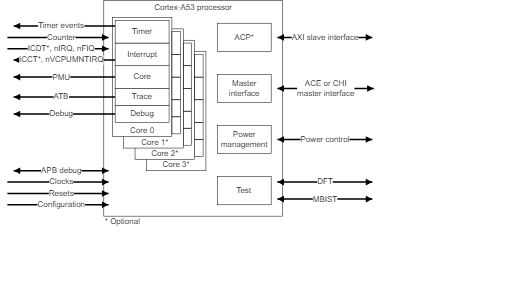
\includegraphics[width=1.0\textwidth]{A53_MPCore_architecture.png}
    \caption{Cortex-A53 MPCore architecture with 4 cores}
\end{figure}

The Cortex-A53 processor is a high efficiency processor that implements the
Armv8-A architecture. While maintaining the A53's energy efficiency, the
Cortex-A53 MPCore enhances overall system performances through parallel
processing.

The A53 CPU has the ability to execute 64-bit applications with the AArch64
execution state. It also has the possibility to execute 32-bit applications
with the AArch32 state for retrocompatibility with the existing ArmV7-A
applications.

\begin{figure}[htb]
    \centering
    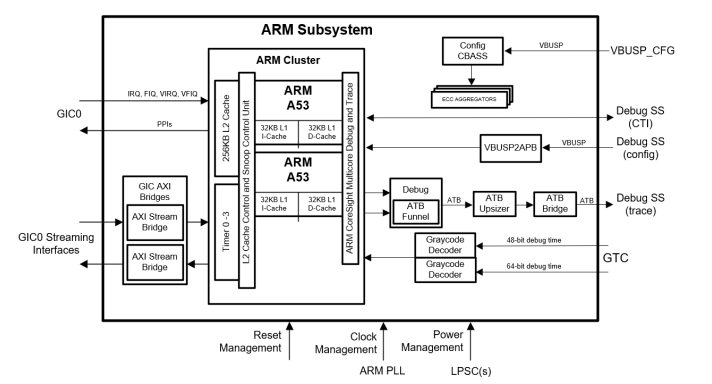
\includegraphics[width=1.0\textwidth]{A53_diagram.png}
    \caption{A53SS Block Diagram}
    \label{fig:A53_diagram}
\end{figure}

Each core within the subsystem is equipped with 32KB L1 instruction and 32KB
L1 data caches, complemented by a shared 256KB L2 cache, as illustrated in
Figure \ref{fig:A53_diagram}. These cache configurations significantly
contribute to optimizing data access and enhancing overall processing
efficiencty.

Given the processing power of the Cortex-A53 core, it is usually used to run
embedded Linux and combine the features offered by Linux with the real-time
operations offered by the other cores.
In this idea, the A53 can be used for general purpose computing and interact
with the other cores to execute certain services which require to satisfy
real-time contraints.

\subsection{R5F Subsystem}

The board selected for the project has two R5F subsystems, a dual-core
implementation of the R5F processor, which is a version of the R5 processor
with the floating point unit extension.

\begin{figure}[ht]
    \centering
    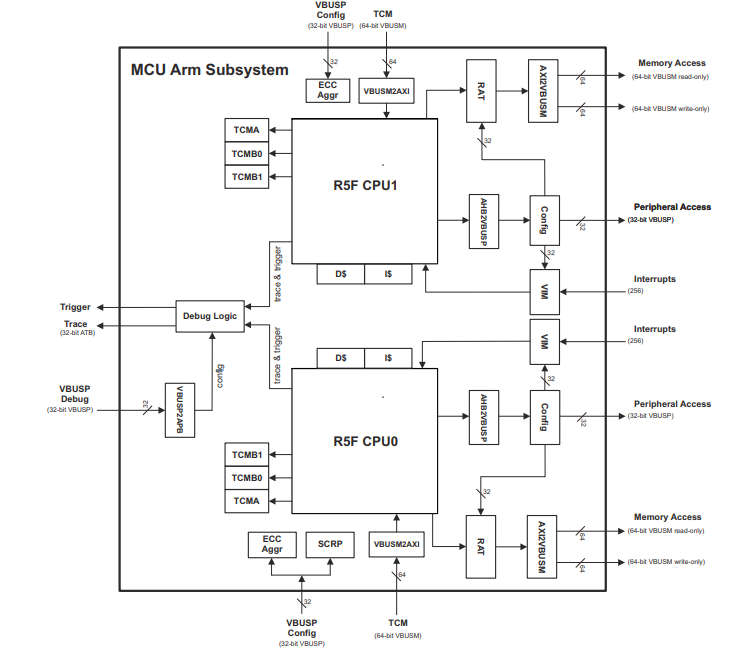
\includegraphics[width=1.0\textwidth]{R5FSS_diagram.png}
    \caption{R5FSS Block Diagram}
\end{figure}

The architecture of the R5F core is the Armv7-R, which is specifically designed
for real-time applications.
The most important features are: deterministic behavior, safety and
reliability.

It features an harvard memory architecture, which separates the cache for
instructions and the cache for data.
Each core has a total of 32KB of L1 cache: 16KB for instruction and 16KB for
data.

To enable fast memory access the R5F has two tightly-coupled memories (TCMs),
which are low latency, tightly integrated memories that can be used for
instructions or data. The total TCM available for each core is of 32KB.
It has the same performance of accessing data instructions or data in cache.
\cite{Technical_reference_AM64}

One of the most important features of the TCMs is the possibility to be
accessed from external sources. This makes possbile to preload data in the
memory, such as instructions before they are needed from the core.
It is also possible to process data and save it on the TCMs, and external
sources can directly access the data, without communicating with the core.

The subsystem can operate in one of two modes: split or single-core mode, which
has to be decided during bootstrap.
In split mode, each core of the subsystem is considered as a standalone
processor, working completely independent from the other, and each of them has
dedicated RAMs and interfaces.
In single-core mode, only one of the cores is operating, but it has available
the TCM of the second core, which could be offered advantages in performance if
the processing power of two cores is not needed, but a lot of data has to be
processed. 

\subsection{M4F Subsystem}


\subsection{PRU-ICSSG}


\section{Inter Processor Communication}


